\chapter{Guida Admin}
\label{app:admin}

Il pannello admin Django del Portale Avifauna deve permettere di controllare ogni passo del sistema. Una volta effettuato il login si accede alla homepage del pannello admin e si può procedere in ogni sezione desiderata attraverso la barra di navigazione verticale a sinistra dello schermo (figura~\ref{fig:admin-navbar}).

\begin{figure}
 \centering
 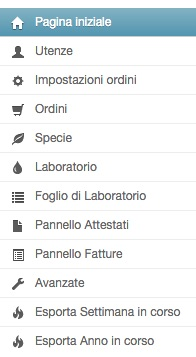
\includegraphics[width=0.25\textwidth]{images/admin-navbar}
 \caption{barra di navigazione laterale nel pannello admin}
 \label{fig:admin-navbar}
\end{figure}

\section*{Utenze}
Per gestire tutti dati diretti che riguardano il cliente è stata creata la sezione \emph{Utenze}, la quale raccoglie gli utenti, i clienti, le associazioni e le iscrizioni ad esse.

Un \textsf{utente} del sistema é un entità identificata da un univoco indirizzo email, con password e nominativo. Esso ha attributi booleani per indicare se é attivo, se ha privilegi di staff o da superutente ed é inoltre possibile indicare i singoli privilegi in un apposito elenco (figura~\ref{fig:admin-utente})..

Un \textsf{cliente} invece é un entità associata ad un utente, con tutti gli attributi personali come nome, cognome, codice fiscale/partita iva, indirizzo, contatti telefonici e attributi di sistema come lo schema prezzi associato, la lingua preferita, la quantità di crediti FEM in possesso e l'eventuale collegamento ad una associazione (figure~\ref{fig:admin-cliente} e~\ref{fig:admin-cliente-tab}).

Le \textsf{associazioni} sono caratterizzate da un nome univoco, uno schema prezzi associato e eventuali informazioni aggiuntive (figura~\ref{fig:admin-associazione}).

Per indicare la correlazione tra cliente ed associazione esiste l'entità \textsf{iscrizione ad associazione} con il nominativo del cliente, l'associazione collegata e il numero di tessera corrispondente.

É stato inoltre aggiunto l'attributo booleano \texttt{ufficiale} per permettere agli addetti di {\fem} di indicare quando l'iscrizione del cliente all'associazione corrisponde al vero, poiché il registro degli iscritti di ogni associazione é aggiornato continuamente ma inviato a {\fem} solo ad intervalli non sempre regolari.

\begin{figure}
 \centering
 \begin{subfigure}[b]{0.69\textwidth}
   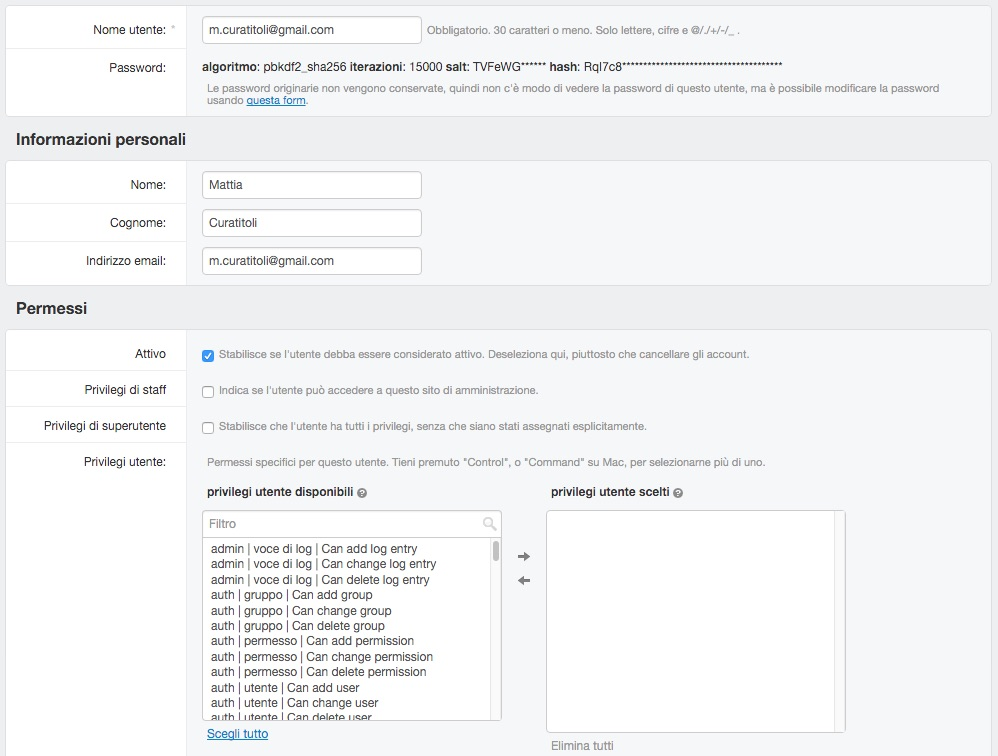
\includegraphics[width=0.95\textwidth]{images/admin-utente} \quad
   \caption{vista di un utente}
   \label{fig:admin-utente}
 \end{subfigure}
 \begin{subfigure}[b]{0.29\textwidth}
   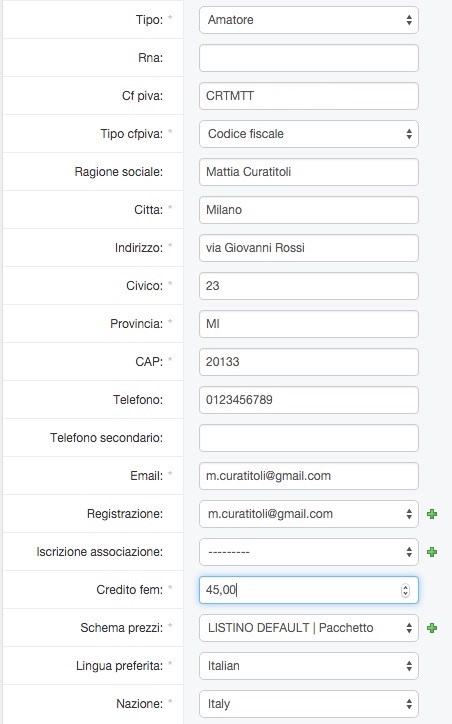
\includegraphics[width=0.95\textwidth]{images/admin-cliente} 
   \caption{vista di un cliente}
   \label{fig:admin-cliente}
 \end{subfigure}
 \begin{subfigure}[b]{1\textwidth}
   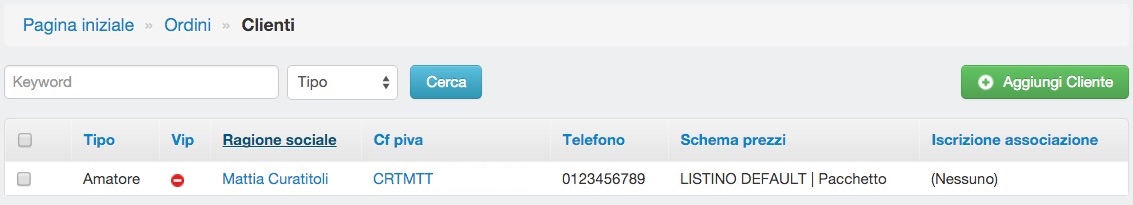
\includegraphics[width=\textwidth]{images/admin-cliente-tab}
   \caption{vista della tabella con l'elenco di clienti registrati}
   \label{fig:admin-cliente-tab}
 \end{subfigure}
 \begin{subfigure}[b]{0.6\textwidth}
   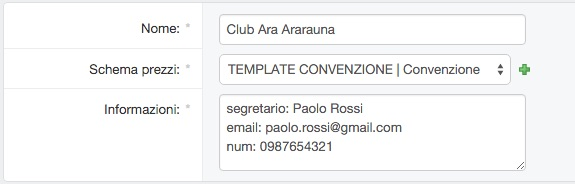
\includegraphics[width=\textwidth]{images/admin-associazione}
   \caption{vista di una associazione}
   \label{fig:admin-associazione}
 \end{subfigure}
 \caption{schermate utenze nel pannello admin}
 \label{fig:admin-utenze}
\end{figure}

\section*{Impostazioni ordini}
Nella sezione \emph{Impostazioni ordini} si trovano quelle opzioni che vengono impostate una tantum e non subiscono frequenti variazioni o controlli.

Vengono raccolti gli \textsf{schemi di prezzi} creati, indicati dal nome e contenenti le tariffe di ogni analisi e attestato. Essi hanno la possibilità di essere di due tipi: Convenzioni o Pacchetti. 

Nel primo caso (tipico di associazioni o clienti professionisti che analizzano un range di specie ridotto) vengono impostati i costi delle analisi come convenzionati, l'ulteriore costo scontato in caso di superamento di una soglia minima dell'ordine e la soglia da superare; vengono anche elencate le specie sulle quali effettuare i prezzi favorevoli e quali invece mantengono il prezzo di listino (figura~\ref{fig:admin-convenzione}).

Nel secondo caso invece vanno impostati anche i prezzi scontati di tutte le analisi da applicare in caso di combinazione tra più analisi richieste sullo stesso soggetto (figura~\ref{fig:admin-pacchetto}).

\begin{figure}
 \centering
 \begin{subfigure}[b]{0.49\textwidth}
   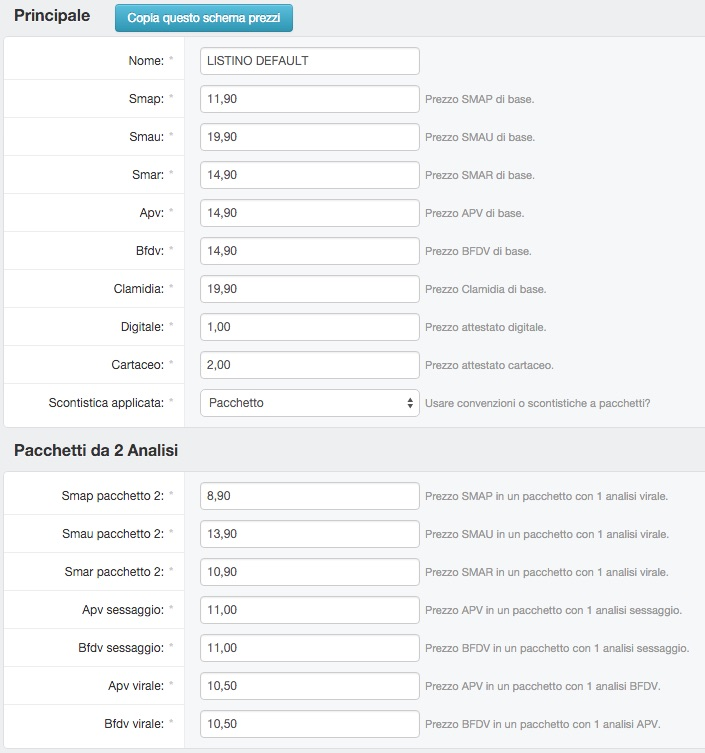
\includegraphics[width=\textwidth]{images/admin-pacchetto} 
   \caption{schema prezzi di tipo pacchetto}
   \label{fig:admin-pacchetto}
 \end{subfigure}
 \begin{subfigure}[b]{0.49\textwidth}
   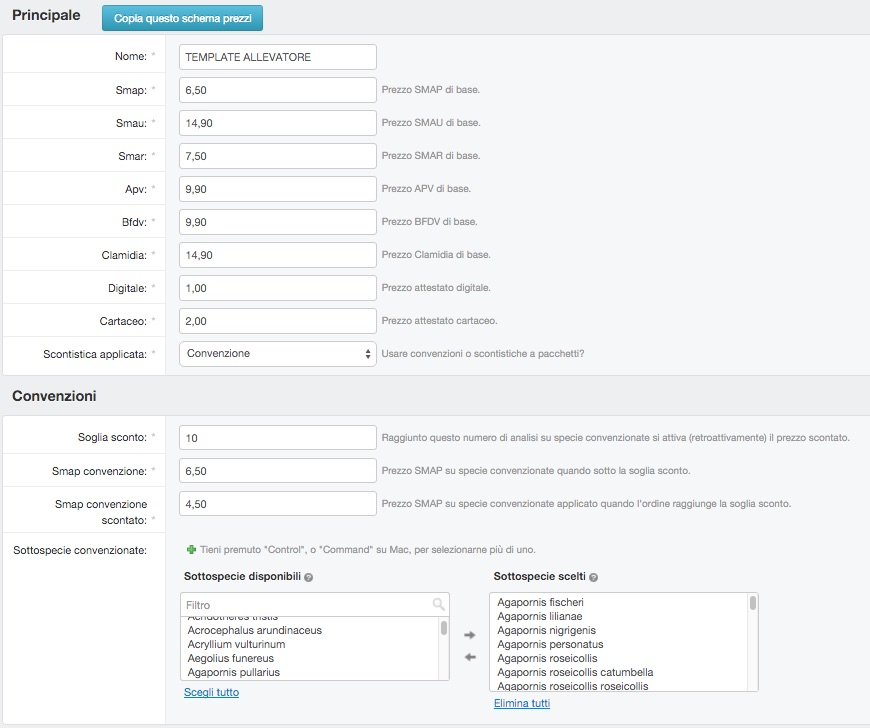
\includegraphics[width=\textwidth]{images/admin-convenzione} 
   \caption{schema prezzi di tipo convenzione}
   \label{fig:admin-convenzione}
 \end{subfigure}
 \caption{schermate di impostazione schema prezzo}
 \label{fig:admin-schema-prezzi}
\end{figure}

In un altra sottosezione (\emph{Pacchetti crediti}) sono indicate le cifre dei \textsf{pacchetti crediti FEM} acquistabili, ovvero il prezzo di ciascuno e il credito che il cliente accumula acquistandolo.

Infine si possono impostare e modificare i \textsf{template messaggi}, cioè i messaggi pre-popolati che sono utilizzati nelle fasi di invio comunicazioni automatiche. Ogni template messaggio ha un nome identificativo univoco, descrizione e ordinamento opzionali e i corpi del testo divisi per ogni lingua (figura~\ref{fig:admin-template-mess}).

\begin{figure}
 \centering
 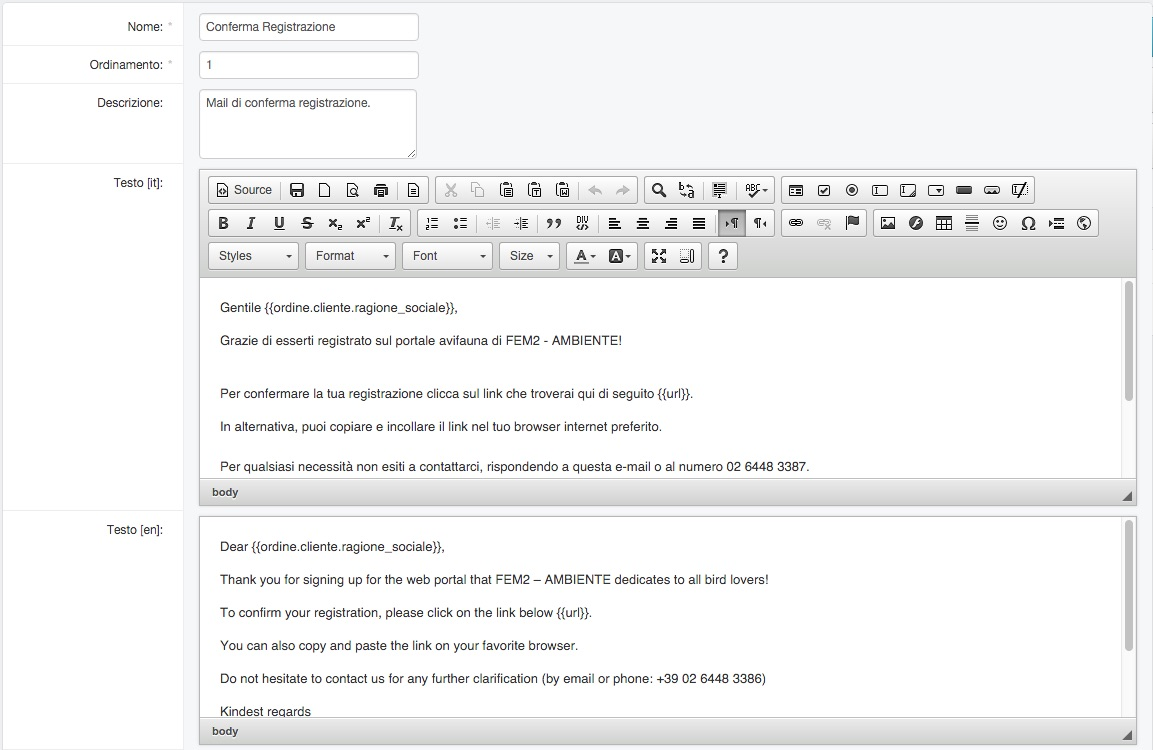
\includegraphics[width=0.75\textwidth]{images/admin-template-mess}
 \caption{vista messaggio template}
 \label{fig:admin-template-mess}
\end{figure}

\section*{Ordini}
Gli \textsf{ordini} sono descritti da campi non modificabili come il suo stato, l'ammontare e il cliente associato; contengono note fiscali o interne e mostrano la lista di campioni associati con la possibilità di indicare eventuali problematiche di ogni singolo campione. Viene fornita la possibilità di assegnare un \texttt{idLab} (numero sequenziale per il laboratorio) ad ogni campione in modo da procedere con le analisi con un apposito tasto (figura~\ref{fig:admin-ordine}). 

É anche possibile comunicare direttamente con il cliente attraverso l'apposito tasto \texttt{Messaggi} che apre un editor WYSIWYG (acronimo dall'inglese What You See Is What You Get) ovvero un editor testuale per la scrittura istantanea ed immediata di un messaggio diretto al cliente (figura~\ref{fig:admin-ordine-mess}).

\begin{figure}
 \centering
 \begin{subfigure}[b]{0.75\textwidth}
   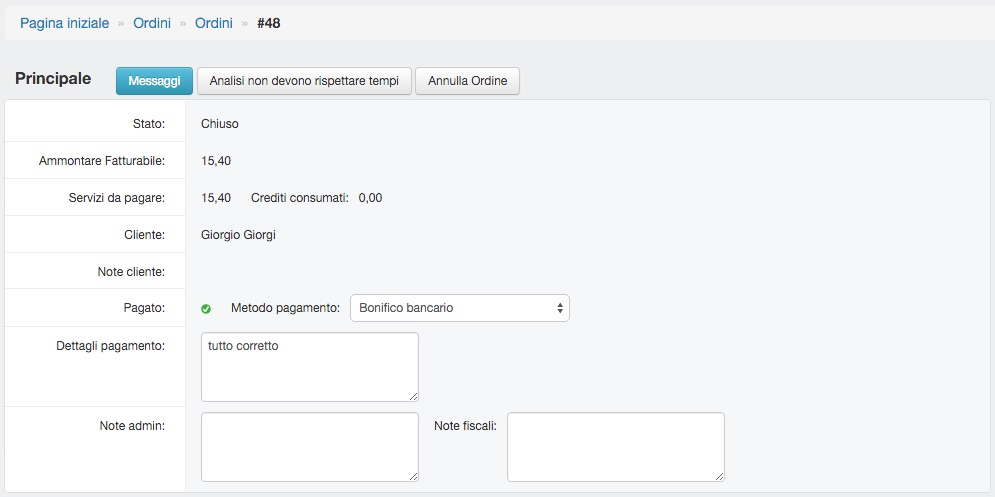
\includegraphics[width=\textwidth]{images/admin-ordine-p} 
   \caption{vista principale dell'ordine}
 \end{subfigure}
 \begin{subfigure}[b]{0.75\textwidth}
   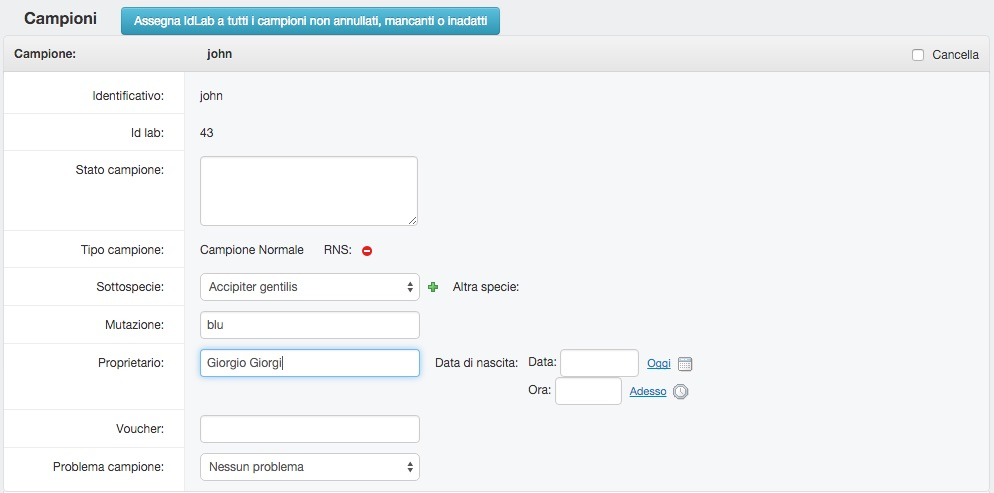
\includegraphics[width=\textwidth]{images/admin-ordine-c}
   \caption{vista dei campioni dell'ordine}
 \end{subfigure}
 \begin{subfigure}[b]{0.4\textwidth}
   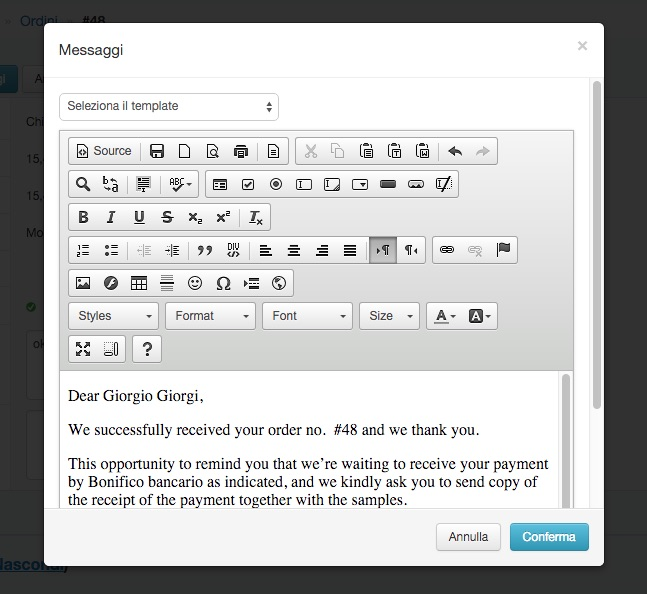
\includegraphics[width=\textwidth]{images/admin-ordine-mess} 
   \caption{modale con l'editor per l'invio di un messaggio diretto}
   \label{fig:admin-ordine-mess}
 \end{subfigure}
 \caption{viste di un ordine}
 \label{fig:admin-ordine}
\end{figure}

La sezione \textsf{campioni} permette una vista completa di tutti i campioni richiesti da analizzare in una tabella in cui viene indicato il numero dell'ordine di ciascun campione, l'identificativo e la specie. É possibile inoltre modificare alcune informazioni del campione per andare incontro ad eventuali errori di battitura.

In \textsf{acquisto crediti} é possibile visualizzare tutte le transazioni relative all'acquisto di pacchetti crediti FEM ed eventualmente effettuare modifiche.

\section*{Specie}
La possibilità di aggiornare la lista di \textsf{specie} e \textsf{sottospecie} é essenziale per il continuo aggiornamento e sviluppo del lavoro di analisi da parte di {\fem}; per renderlo possibile in una sezione apposita del pannello admin sono elencate tutte le specie e sottospecie presenti, con la possibilità di aggiornare, modificare e completare le relative informazioni, tra cui i nomi comuni e le immagini.

\section*{Laboratorio}
La sezione dedicata al \emph{laboratorio} é uno dei punti cruciali in cui viene svolto la maggior parte del lavoro da parte dei tecnici di {\fem}; é infatti necessario elencare tutte le analisi da eseguire riferite ai relativi campioni, aggiungendo informazioni specifiche come i metodi di estrazione ed amplificazione del DNA in funzione all'analisi richiesta (figura~\ref{fig:admin-analisi-tab}). 

Essendo un ambito ancora in fase di ricerca non é detto che una metodologia scelta corrisponda per forza alla migliore, per questo motivo sono state create le sezioni \textsf{metodo estrazione}, \textsf{metodo amplificazione}, \textsf{metodo visualizzazione} per effettuare i dovuti aggiornamenti. Sono stati inoltre inseriti tre campi di tipo \tag{select} in ogni analisi per permettere ai tecnici di cambiare la metodologia scelta in caso di nuove sperimentazioni. É stato creato per questo il meccanismo del 'processamento multilplo' che permette di effettuare più volte la stessa analisi su un campione, archiviando i dati relativi a ciascun processamento (figura~\ref{fig:admin-analisi}). 

É importante questa struttura per la creazione del \textsf{foglio di laboratorio}.

\begin{figure}
 \centering
 \begin{subfigure}[b]{0.85\textwidth}
   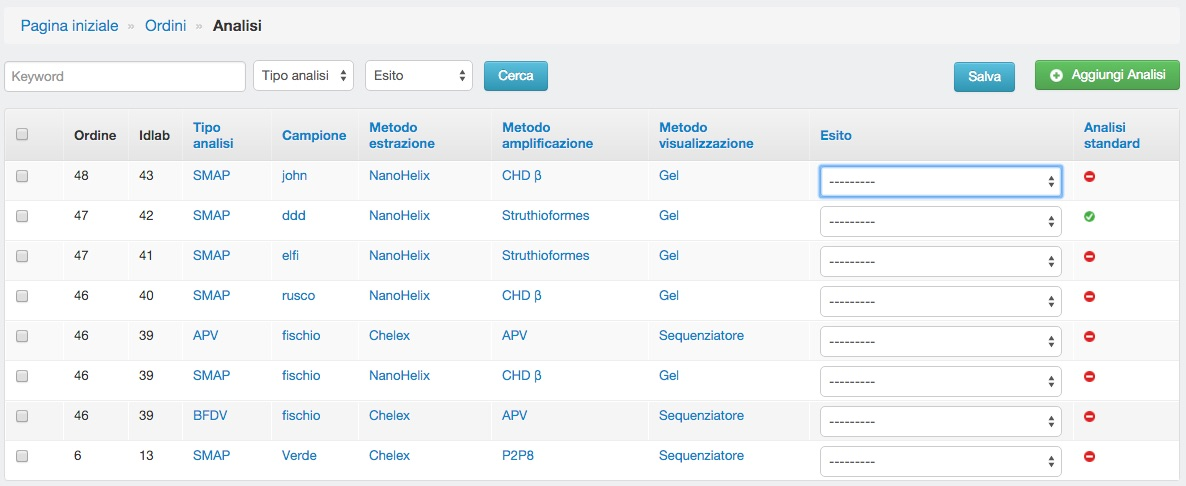
\includegraphics[width=\textwidth]{images/admin-analisi-tab} 
   \caption{elenco di analisi}
   \label{fig:admin-analisi-tab}
 \end{subfigure}
 \begin{subfigure}[b]{0.55\textwidth}
   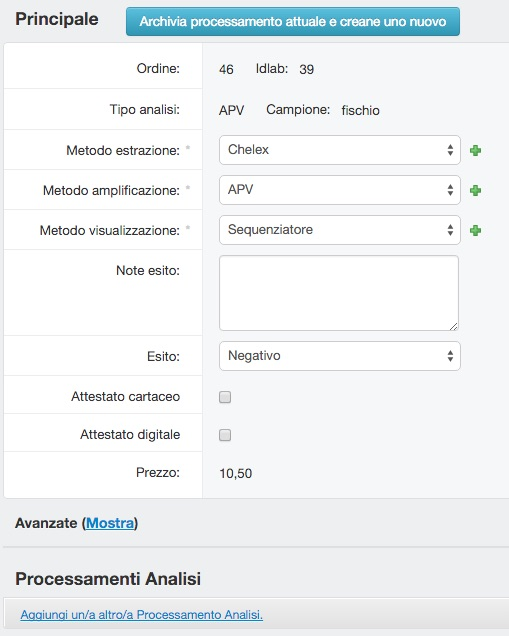
\includegraphics[width=\textwidth]{images/admin-analisi}
   \caption{vista analisi singola}
   \label{fig:admin-analisi}
 \end{subfigure}
 \caption{viste di analisi}
\end{figure}

\section*{Foglio di laboratorio}
Il \textsf{foglio di laboratorio} é una tabella dinamica creata in una sezione apposita del pannello admin, che viene popolata esclusivamente con le analisi ancora da effettuare (cioè che non hanno un esito finale già stabilito).

Questa tabella oltre ad indicare informazioni classiche come l'identificativo del campione, il numero dell'ordine di riferimento e il numero progressivo di laboratorio (idLab), indica con precisione la specie, le analisi da effettuare e le metodologie consigliate, lasciando uno spazio per le note da inserire durante il processamento. Essa viene stampata dal tecnico attraverso l'apposito tasto che genera un pdf e tramite codice {\js} apre una finestra di dialogo diretta per la stampa (figura~\ref{fig:admin-fogliolab}).

\begin{figure}
 \centering
 \begin{subfigure}[b]{0.95\textwidth}
   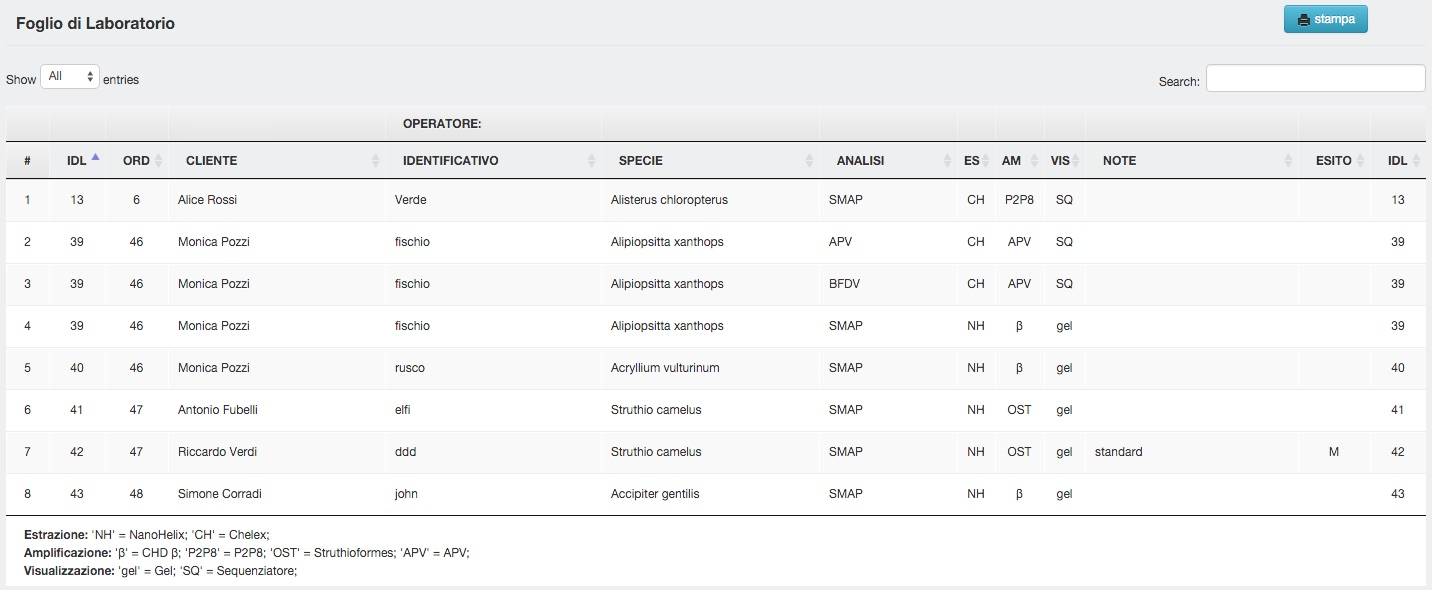
\includegraphics[width=\textwidth]{images/admin-fogliolab-tab} 
   \caption{tabella per il foglio di laboratorio}
 \end{subfigure}
 \begin{subfigure}[b]{0.95\textwidth}
   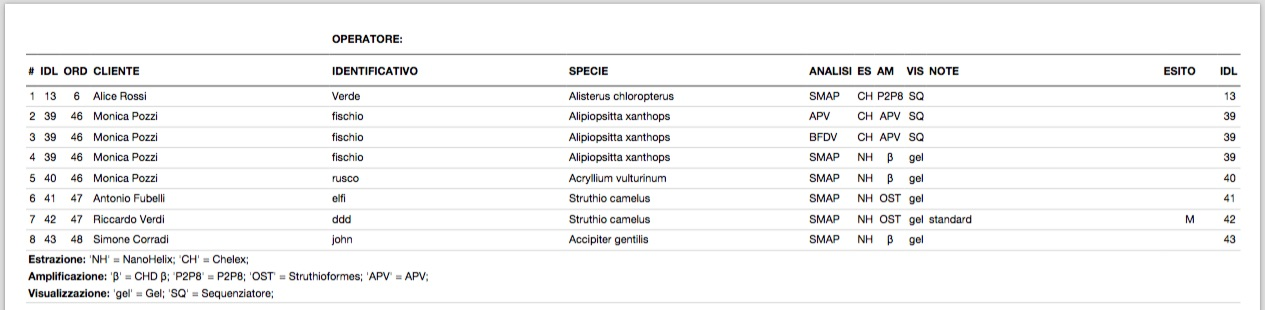
\includegraphics[width=\textwidth]{images/admin-fogliolab}
   \caption{estratto del foglio di laboratorio cartaceo generato}
 \end{subfigure}
 \caption{generazione foglio di laboratorio}
 \label{fig:admin-fogliolab}
\end{figure}

\section*{Pannello attestati e Pannello fatture}
I pannelli di attestati e fatture sono tabelle semplici ed analoghe al foglio di laboratorio che però servono nelle fasi finali del flusso di ogni ordine.

Il \textsf{pannello attestati} elenca gli ordini che richiedono una stampa cartacea degli attestati per la successiva spedizione tramite posta, offre la creazione dinamica degli attestati in questione e la possibilità di tenere traccia di quelli mancanti.

Il \textsf{pannello fatture} è molto simile e tiene traccia degli ordini per cui é già stata emessa fattura.

\section*{Avanzate ed Esporta}
La sezione \textsf{Avanzate} permette modifiche nelle coordinate dei pagamenti PayPal. 

I tasti per l'\textsf{esportazione} invece permettono la creazione e download di file in formato \texttt{.csv}, ovvero file testuali per la costruzione di tabelle, nelle quali il sistema inserisce alcuni dati scelti da {\fem} utili per le statistiche.
